\section{Durchführung}
\label{sec:Durchführung}
\subsection{Ablenkung im elektrischen Feld}
    Im ersten Versuchsteil wird die Ablenkung der Elektronen im elektrischen Feld untersucht. Dazu wird die Schaltung aus 
    \autoref{fig:schaltung1} verwendet. Es werden nun fünf veschiedene Beschleunigungsspannungen im Bereich von $180$V bis $500$V
    angelegt. Die Ablenkspannung, welche am 
    Voltmeter abzulesen ist, wird so eingestellt, dass die Elektronen, nacheinander auf die neun äquidistanten Linien des auf dem 
    Detektorschirm angebrachten Koordinatennetzes fallen. Diese Ablenkspannungen werden notiert. Dabei ist darauf zu achten, dass der 
    zusehende Leuchtfleck keine große Ausdehenung hat. Des Weiteren wird der Abstand der neun Linien voneinander gemessen und ebenfalls notiert.
    \begin{figure}
        \centering
        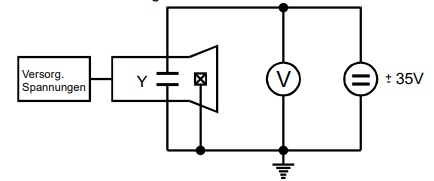
\includegraphics[width=0.7\textwidth]{content/schaltung_ablenk.png}
        \caption{Schaltskizze zur Untersuchung des Zusammenhanges zwischen Beschleunigungsspannung und Verschiebung auf dem Detektorschirm \cite{V501-und-V502}.}
        \label{fig:schaltung1}
    \end{figure}


    Anschließend wird die Schaltung aus \autoref{fig:schaltung2} verwendet. Hierbei soll der in \autoref{sec:oszillo} aufgestellte
    Zusammenhang zwischen der Frequenz der Sägezahnspannung und einer angelegten Sinusspannung untersucht werden. 
    Bei konstanter Beschleunigungsspannung von werden vier verschieden Vielfache ($n = \frac{1}{2}, 1, 2, 3$) der Sinusspannung untersucht
    und die zugehörigen Frequenzen der Sägezahnspannung notiert, bei denen ein stehendes Bild einer Sinuswelle zu sehen ist.
     \begin{figure}
        \centering
        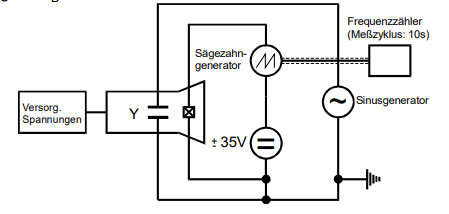
\includegraphics[width=0.7\textwidth]{content/wechselschaltung.png}
        \caption{Schaltskizze zur Untersuchung des Zusammenhangs von Sägezahn- und angelegter Wechselspannung \cite{V501-und-V502}.}
        \label{fig:schaltung2}
    \end{figure}
    \subsection{Ablenkung im magnetischen Feld}
    Im zweiten Versuchsteil wird das Kathodenstrahlrohr in die Mitte eines Helmholtzspulenpaares, welches dort ein weitgehend homogenes Magnetfeld
    erzeugen kann, gebracht. Die technischen Daten des Spulenpaares sind zu notieren. Zu beachten ist, dass die Achse der Kathodenstrahlröhre in 
    Richtung der Horizontalkomponente des Erdmagnetfeldes ausgerichtet wird. Zur Bestimmung dieser wird ein Deklinatorium-Inklinatorium
    verwendet. Das durch das Helmholtzspulenpaar erzeugte Magnetfeld kann durch eine Stromquelle eingestellt werden. Es soll nun für die 
    konstanten Beschleunigungsspannungen $250$V und $400$V, die Auslenkung in Abhängigkeit von der Stromstärke bestimmt werden. 
    Hierzu werden wie zuvor die neun äquidistanten Linien am Kathodenstrahlrohr verwendet und die zugehörigen Stromstärken notiert.
    Dabei muss der Elektronenstrahl aber zunächst bei einer Stromstärke von $0$A auf die erste Linie gebracht werden.
    
    Anschließend wird die Intensität des Erdmagnetfeldes am Ort des Versuchs untersucht. Mittels des Inklinatoriums wird dazu zunächst der
    Inklinationswinkel bestimmt. Dieser ist der Winkel zwischen der Horizontalebene und der Richtung des Magnetfeldes. Hierzu wird das 
    Inklinatorium in Nord- beziehungsweise Südrichtung ausgerichtet und anschließend um $90°$ gekippt. Die Nadel zeigt nun in Richtung des
    Erdmagnetfeldes. Dieser Winkel wird notiert. Des Weiteren wird das Kathodenstrahlrohr bei ausgeschaltetem Magnetfeld so eingestellt, dass
    der Elektronenstrahl auf einen Punkt trifft, welcher leicht ablesbar ist. Dieser Punkt wird sich gemerkt. Der gesamte Aufbau wird nun um $90°$,
    sodass das Kathodenstrahlrohr in Ost-/Westrichtung zeigt. Der Elektronenstrahl wird nun auf eine andere Postion treffen. 
    Das Magnetfeld wird nun aktiviert und der Strom so geregelt, dass der Elektronenstrahl 
    wieder auf die vorherige Position trifft. Der Wert der Stromstärke wird notiert.